% !Mode:: "TeX:UTF-8" 

\BiChapter{结论与展望}{Conclusions and Future Works}\label{chap6}

\BiSection{工作总结与主要成果}{The Summary and Main Results}\label{chap61}

网络通信是构建当今社会的重要基础设施,现代网络在向软件定义、数据平面可编程的方向发展。网络架构变迁的核心是有一套可编程的可以映射上层控制逻辑的硬件数据平面。本文主要探索编程硬件的网络系统,使其能够满足快速迭代的网络创新需求,在能够提供与现阶段匹配的处理性能的同时兼顾系统安全性。

本文从网络系统的三个维度进行分析:(1)主机侧网络,在服务器网卡层面,基于 CPU 的智能网卡性能难以满足目前虚拟化技术和网络监管细粒度化的发展需
求。(2)交换侧网络,在核心网骨干网层面,基于 ASIC 的转发平面不足以提供网络处理的高灵活性。由于在成本、性能之间平衡困难,网络工程师的创新空间受到了限制。(3)控制面与数据面交互,硬件流表是一种高效且昂贵的网络转发核心部件,在软件定义网络时代流表稀缺性更加突出。由于流数目和流量的快速增长,控制平面针对流表的操作导致大量控制通信开销。易导致网络鲁棒性差,易形成安全隐患。
现场可编程门阵列(FPGA)器件得到快速发展,以可编程硬件技术为首的异构架构已经大量融合到网络领域,带来高用户可定制能力的同时也能保证了一定的处理性能。

第一,SDN网络硬件流表可扩展性研究。由可编程网卡和交换机组成的数据平面内,最重要的资源是流表资源。本文从SDN网络全局视野出发,着手解决流表资源匮乏的问题。本文分析不同的流量规模和特征,以及系统多模块之间的互联协议,提出一种转发设备节点之间的流表共享机制。本文基于流量分布规律以及理论分析,提出了流表共享机制FTS,扩展了OpenFlow交换机的Table-Miss处理方式。可以有效地缓解流表溢出现象带来的巨大网络通信性能损失,实现了数据平面应对突发流量时的稳定性。


第二,本文为增强数据平面转发设备的网络随路计算能力,提出了一种自适应交换系统(Adaptive Switch Architecture, AS)。AS通过保留ASIC交换芯片中的交换网络结构以确保高性能,并且将网络数据可编程性卸载到FPGA可编程硬件中。本文在AS架构中实现了三种难以在目前交换系统中实现的例子,集中体现了AS架构可为目前的交换芯片带来极高的灵活性。此外,本文设计了资源消耗可控的多级并行流水线,并使以上三个应用达到了数个Tbps的吞吐性能。在资源消耗可控的前提下,大规模提高可编程网络数据平面的包处理吞吐性能。

第三,本文研究可编程设备加速主机侧可编程网络的方法。论文将测量系统的可编程性抽象为基础的包个数统计和数据量缩统计方法。
系统包括数据包捕获功能、测量系统和发送引擎。
通过不同的软件调用,令系统硬件适用于高性能的网络安全、访问控制、流量控制、拥塞探测等多种场景。
同时利用基于硬件的存储压缩算法,在节约38\%的硬件存储空间情况下,相较于软件的处理方式系统吞吐率提升8倍、系统的处理能耗节约90\%。在满足网络功能不改变的前提下,证明利用基于 FPGA 的智能网卡能有效地提升服务器的网络性能、降低抖动和提高效率。



综上全文,论文完成了对于可编程数据平面在网络各个层次中的性能优化、灵活性提升以及安全性保障。





\BiSection{研究内容展望}{Future Works}\label{chap62}

\BiSubsection{数据平面可编程网络}{Data of Plane Programmable Network}\label{chap621}

开放的网络数据平面概念已经催生出了新一轮的网络创新热潮,软件定义网络由数据平面控制平面分离转向全可定制化方向发展。学术界在可编程数据平面议题内探讨了大量的新应用新方法,为可编程数据平面展开了光明的发展前途。产业界在可编程数据平面的性能提升上持续耕耘。二者互相促进,为开放网络数据平面的标准化打下坚实的基础。

可编程数据平面中性能与灵活性是一对主要的矛盾,不同的需求场景下选取不同的实现方法,都体现了对这两方面的折中。本文发现异构的架构最终才有可能平衡各方面的需求。现场可编程门阵列是一种通用的数字逻辑技术,它可以实现完整的可编程能力。但受限于FPGA的架构,在网络处理中其性能并不占优。如何设计一种为网络专用的可编程硬件逻辑技术,来彻底解决性能与灵活的矛盾点,也许会成为一个崭新的方向。
但这需要大量网络、芯片技术研究人员共同努力,也需要提升芯片制造和设计能力,是一个庞大的系统工程。




\BiSubsection{网络资源与计算能力}{Network Resources and In-Network Computing}\label{chap622}

\begin{figure}[!ht]
	\centering 
	\vspace{-1.5mm} 
	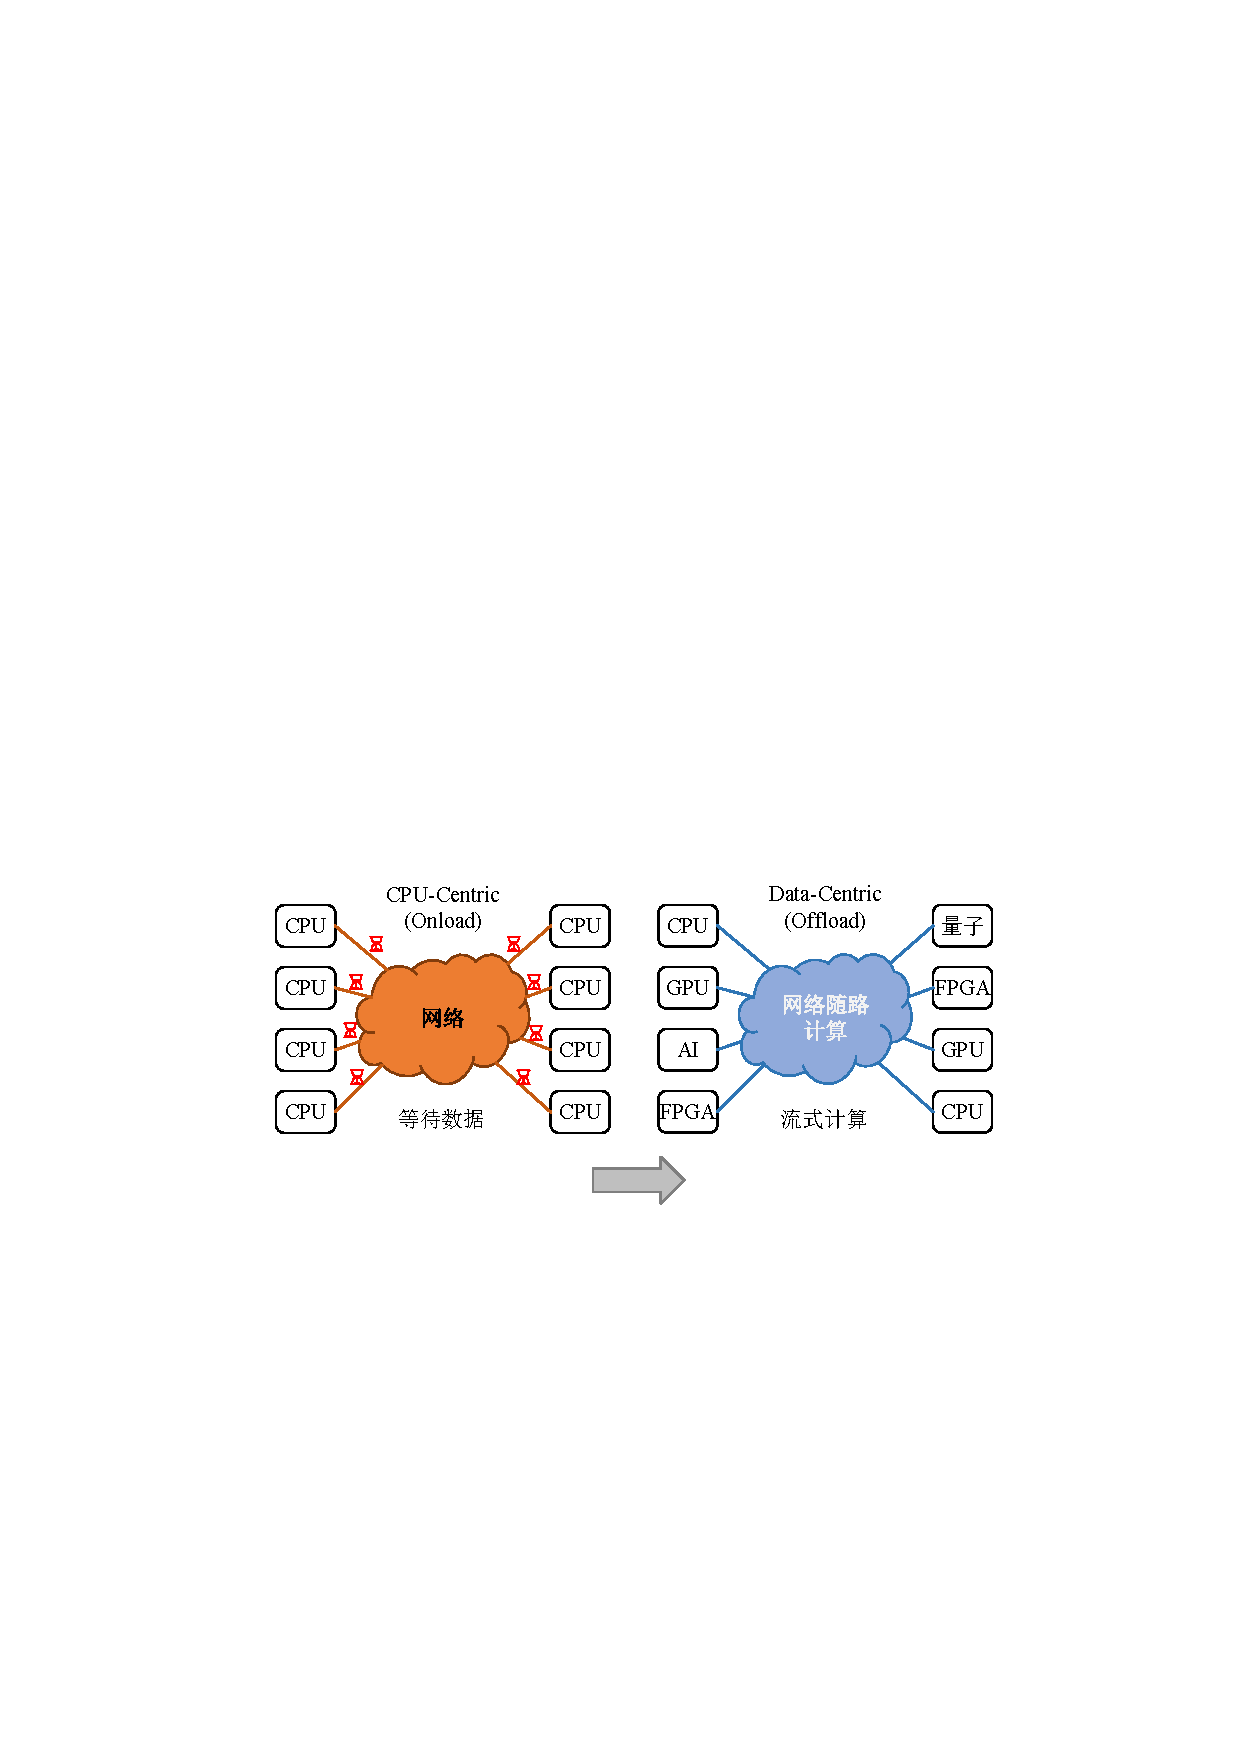
\includegraphics[scale=1]{innetcompute.pdf}
	\caption{网络与计算的深度融合} \label{fig:innetcompute}
\end{figure}

今后,网络不只是承载通信功能,它还是一个对信息进行融合、智能计算和分发的整体设施。网络当中依然有方方面面的问题需要解决,例如转发时延、流量吞吐、网络随路计算等。不同问题的解决,都需要提出一种新的网络架构。对于转发时延和吞吐敏感的应用,人们利用CDN(内容分发网络)和边缘计算来提升信息的快速可达性。对于计算能力来说,由于摩尔定律失效,人们不可能只依靠简单堆叠CPU来满足需求。异构计算(GPU、FPGA、ASIC)一方面是解决未来计算量增长的重要途径,另外也是有效控制服务器数量规模的重要手段。让专业的设备处理专用任务这种概念也变得越来越清晰。网络在这种变化当中也可以起到粘合剂的效果,如图~\ref{fig:innetcompute}~所示,AI应用以及训练任务要求网络提供快速和高效的数据转发,传统以分布式CPU为核心的网络体系中等待数据传输的过程拉低了整体处理效率。网络随路计算、流式计算的概念都给网络应用加速提供了不同的可选车道。以各种不同计算技术(异构计算、量子信息计算)为核心,网络会智能化地指导数据流的最佳流动路径。网络的可编程化由最初的数据平面可编程变为了最终对计算库和数据包处理流程的可编程。










